% Jacobs Portrait Poster
% LaTeX Template
% Version 1.0 (31/08/2015)
% (Based on Version 1.0 (29/03/13) of the landscape template
%
% Created by:
% Computational Physics and Biophysics Group, Jacobs University
% https://teamwork.jacobs-university.de:8443/confluence/display/CoPandBiG/LaTeX+Poster
% 
% Further modified by:
% Nathaniel Johnston (nathaniel@njohnston.ca)
%
% Portrait version by:
% John Hammersley
%
% The landscape version of this template was downloaded from:
% http://www.LaTeXTemplates.com
%
% License:
% CC BY-NC-SA 3.0 (http://creativecommons.org/licenses/by-nc-sa/3.0/)

\documentclass[final]{beamer}

\usepackage[scale=1.24]{beamerposter}

\usetheme{confposter}
\newlength{\sepwid}
\newlength{\onecolwid}
\newlength{\twocolwid}
\newlength{\threecolwid}
\setlength{\paperwidth}{36in}
\setlength{\paperheight}{48in}
\setlength{\sepwid}{0.024\paperwidth}
\setlength{\onecolwid}{0.22\paperwidth}
\setlength{\twocolwid}{0.464\paperwidth}
\setlength{\threecolwid}{0.708\paperwidth}
\setlength{\topmargin}{-0.5in}

\usepackage{booktabs}
\usepackage{graphicx}
\usepackage{natbib}
\usepackage{tikz}
\usetikzlibrary{calc}

\newcommand{\EE}{\mathbb{E}}
\newcommand{\PP}{\mathbb{P}}
\newcommand{\RR}{\mathbb{R}}
\newcommand{\ZZ}{\mathbb{Z}}
\DeclareMathOperator*{\argmax}{arg\,max}

\title{Rank Verification for Exponential Families}

\author{Kenneth Hung \and William Fithian}

\institute{
University of California, Berkeley \\
{\tt \{kenhung, wfithian\}@berkeley.edu}
}

\begin{document}

\addtobeamertemplate{block end}{}{\vspace*{2ex}}
\addtobeamertemplate{block alerted end}{}{\vspace*{2ex}}

\setlength{\belowcaptionskip}{2ex}
\setlength\belowdisplayshortskip{2ex}

\begin{frame}[t]

\begin{columns}[t]

\begin{column}{\sepwid}\end{column}

% column 1
\begin{column}{\onecolwid}

\begin{alertblock}{Objectives}

We extend the classical result on Comparison with Sample Best (CSB) in \citet{Stefansson:1988wj} to a general class of exponential families. We provide procedures for the following three inferences:
\begin{enumerate}
	\item Is the sample best ({\em winner}) the true best ({\em best})?
	\item By how much is the same best better than the rest?
	\item Is the sample second ({\em runner-up}) the true second ({\em second best}), the sample third the true third, etc.?
\end{enumerate}

\end{alertblock}

\begin{block}{Introduction}

\begin{table}[htbp]
\centering
\begin{tabular}{c c c c}
	\hline
	Rank & Candidate & Result & Votes \\
	\hline
	$1$ & Trump & $31\%$ & $276$ \\
	$2$ & Cruz & $24\%$ & $214$ \\
	$3$ & Rubio & $17\%$ & $151$ \\
	$4$ & Carson & $8\%$ & $71$ \\
	$5$ & Paul & $4\%$ & $36$ \\
	$6$ & Bush & $4\%$ & $36$ \\
	$7$ & Huckabee & $3\%$ & $27$ \\
	$\vdots$ & $\vdots$ & $\vdots $ & $\vdots$ \\
	\hline
\end{tabular}
\caption{Simplified results from a February 1, 2016 Quinnipiac University poll of $890$ Iowa Republicans. We assume that the number of votes follows a multinomial distribution.}
\label{tbl:poll}
\end{table}

Questions that one might ask, {\em post hoc}:
\begin{enumerate}
	\item Verifying winner as best: Does Trump have the largest support? (a.k.a.\ multiple comparison with sample best (CSB) in \citet{Stefansson:1988wj})
	\item By how much: How much larger is Trump's support compared to other candidates?
	\item Verifying other ranks: Does Cruz (Rubio, etc.) have the second (third, etc.) largest support?
\end{enumerate}

\end{block}

\begin{block}{Selected Related Work}

\begin{itemize}
	\item Test and lower bound for log-concave location families, using partition principle from \citet{Finner:2002ju}: \citet{Stefansson:1988wj}
	\item Multinomial families: \citet{Gupta:1967wg}
	\item Conditional selective inference: \citet{Fithian:2014ws}
\end{itemize}

\end{block}

\end{column}

\begin{column}{\sepwid}\end{column}

% column 2
\begin{column}{\onecolwid}

\begin{block}{Challenges}

\begin{itemize}
	\item {\em Multiple comparison}: Comparing the winner to the rest involves $n-1$ pairwise comparisons.
	\item {\em Selective inference}: We will only test the hypothesis about the winner, and the winner depends on the sample.
\end{itemize}

\end{block}

\begin{block}{Schur-Concave Exponential Families}

Canonical form exponential families with observations as sufficient statistics:
\begin{align*}
&~ p(x_1, \ldots, x_n; \theta_1, \ldots, \theta_n) \\
= &~ \exp(\theta_1 x_1 + \cdots + \theta_n x_n \\
&~ ~~~~ - \log A(\theta_1, \ldots, \theta_n)) h(x_1, \ldots, x_n)
\end{align*}
\begin{itemize}
\item $x_i$ are the observations
\item $\theta_i$ are the natural parameter being ranked and tested
\item $h(\cdot)$ is the carrier distribution
\item $A(\cdot)$ is the normalizing constant
\end{itemize}

Schur-concave exponential families require $h(\cdot)$ to be Schur-concave, i.e.
\[
h(x) \le h(y) ~~~~ \text{if} ~~~~ x \succeq y,
\]
where $x \succeq y$ is the majorization order in $\RR^n$.

\end{block}

\begin{block}{Examples}

\begin{itemize}
	\item Independent binomial treatment outcomes in a clinical trial
	\item Competitive sports under the Bradley--Terry model
	\item Comparing the variances of independent normal populations
\end{itemize}

\end{block}

\begin{alertblock}{Procedures}

For observations from a Schur-concave exponential family, we provide the following three procedures for the three inferences above:
\begin{enumerate}
	\item {\bf Two}-tailed level-$\alpha$ test comparing winner (Trump) to runner-up (Cruz)
	\item Invert the test above
	\item {\bf Two}-tailed level-$\alpha$ test comparing first runner-up (Cruz) to second runner-up (Rubio), etc., using a stepwise procedure
\end{enumerate}

A two-tailed level-$\alpha$ test here refers to the conditional exact test for exponential families.

\end{alertblock}

\end{column}

\begin{column}{\sepwid}\end{column}

% column 3
\begin{column}{\onecolwid}

\begin{block}{Key Ideas in Proof}

\begin{itemize}
	\item {\em Multiple comparison}: Null hypothesis is ``the winner is not the best'', a union null of hypothesis that the winner is not better than each of the rest
	\item Construct a $p$-value $p_{ij}$ for comparing winner $i$ to each of the rest, $j$; do a significance test based on the combined $p$-value $\max_{j \ne i} p_{ij}$.
	\item {\em Selective inference}: Construct $p_{ij}$ by conditioning on the selection event \citep{Fithian:2014ws}, given by
	\[
	\{X_i > \max_{i \ne k} X_k\}
	\]
	\item Condition also on sufficient statistics for nuisance parameters, $X_{\setminus\{i, j\}}$ and $X_i + X_j$, for an exact test
\end{itemize}

\end{block}

\begin{alertblock}{Goal in Proof}

It suffices to show
\begin{itemize}
	\item $\max_{k \ne i} p_{ik} = p_{ij}$, where $i$ is the winner and $j$ is the first runner-up.
	\item $p_{ij}$ is the $p$-value obtained from a two-sided exact test comparing only winner $i$ and runner-up $j$.
\end{itemize}

\end{alertblock}

\begin{block}{Proof by Picture}
\begin{itemize}
	\item Graphical representation of $p_{ij}$ and $p_{ik}$ for comparison
	\item WLOG assume that $i = 1$ is the winner, $j = 2$ is the runner-up, and $k = 3$ is any other candidate
	\item Under the conditioning, $X_1 + X_2 + X_3$ and $X_{\setminus\{1, 2, 3\}}$ are held constant
	\item Everything can fit on a 2D picture!
\end{itemize}

\centering
\begin{tikzpicture}[scale=1.9,every node/.style={scale=0.7}]
	\coordinate (C1) at (60:5);
	\coordinate (C2) at (300:3);
	\coordinate (A) at (60:3);
	\coordinate (B) at ($(A) + (330:3)$);
	\coordinate (C) at ($(0, 0)!(B)!(C2)$);
	\coordinate (D) at ($(A) + (150:1)$);
	\draw[dashed] (0, 0) -- (C1);
	\draw[dashed] (0, 0) -- (C2);
	\fill[byzantium!50] (0, 0) -- (C1) -- ($(C1) + (6.5, 0)$) -- ($(C2) + (7.5, 0)$) -- (C2) -- cycle;
	\node[above left] at ($(C2) + (7.5, 0)$) {$A_1$};
	\draw[thick] (A) -- (B) node[midway, above right] {$A$};
	\draw[thick, ->] (B) -- ++(330:5) node[midway, below left] {$B$};
	\fill (A) circle(2pt) node[above right] {$\left(M_{12}, M_{12}, X_3\right)$};
	\fill (B) circle(2pt) node[right] {$\left(X_1, X_2, X_3\right)$};
	\fill (0, 0) circle(2pt);
	\draw[thick, ->] (0, 0) -- (0.5, 0) node[right] {\scriptsize $x_1 +$};
	\draw[thick, ->] (0, 0) -- (120:0.5) node[above] {\scriptsize $x_2 +$};
	\draw[thick, ->] (0, 0) -- (240:0.5) node[below] {\scriptsize $x_3 +$};
	\draw[thick] (C) -- (B) node[midway, below right] {$C$};
	\node[below] at (C) {$\left(M_{13}, X_2, M_{13}\right)$};
	\draw[thick, ->] (B) -- ++(30:5) node[midway, above left] {$D$};
	\fill ($(0, 0)!(B)!(C2)$) circle(2pt);
	\draw[thick, dashed] (A) -- (D) node[midway, below left] {$\tilde{A}$};
	\fill (D) circle(2pt) node[above] {$\left(M_{13}, X_2 + D_{13}, X_3\right)$};
	\draw[thick, dotted] (C) -- (D) node[midway, below, rotate=-90] {$\succeq$};
	\draw[thick, dotted] (A) -- ++(0, -3) node[midway, below, rotate=-90] {$\succeq$};
	\draw[thick, dotted] ($(B) + (30:4)$) -- ($(B) + (330:4)$) node[midway, below, rotate=-90] {$\succeq$};
\end{tikzpicture}

\begin{itemize}
	\item $p_{12} = \frac{B}{A+B}$ and $p_{13} = \frac{D}{C+D}$
	\item Schur concavity implies $A + \tilde{A} \le C$ and $D \le B$
	\item So $p_{12} \ge p_{13}$
	\item The values are symmetric about the $x_1 = x_2$ line, so $\frac{B}{A+B}$ is equivalent to a two-tailed $p$-value.
\end{itemize}

\end{block}

\end{column}

\begin{column}{\sepwid}\end{column}

% column 4
\begin{column}{\onecolwid}

\begin{block}{Brief Sketch for Other Two Inferences}

\begin{itemize}
	\item A test can be built, similarly for the hypothesis that winner is not at least $\delta$ larger than the rest; inverting this test yields the second procedure
	\item Adopting the framework in \citet{Fithian:2015uj}, we can perform a sequence of similar selective inferences
\end{itemize}

\end{block}

\begin{block}{Power Comparison}

\begin{itemize}
\item \citet{Gupta:1967wg} provided a subset selection procedure for the multinomial problem
\item Convert into a test for if the winner is the best by rejecting the null hypothesis if only the winner is selected
\item Tested on parameters in form of
\[
\text{prob} \propto (e^\delta, \underbrace{1, 1, \ldots, 1}_{n - 1}), ~~~~ \text{num} = m
\]
\end{itemize}

\centering
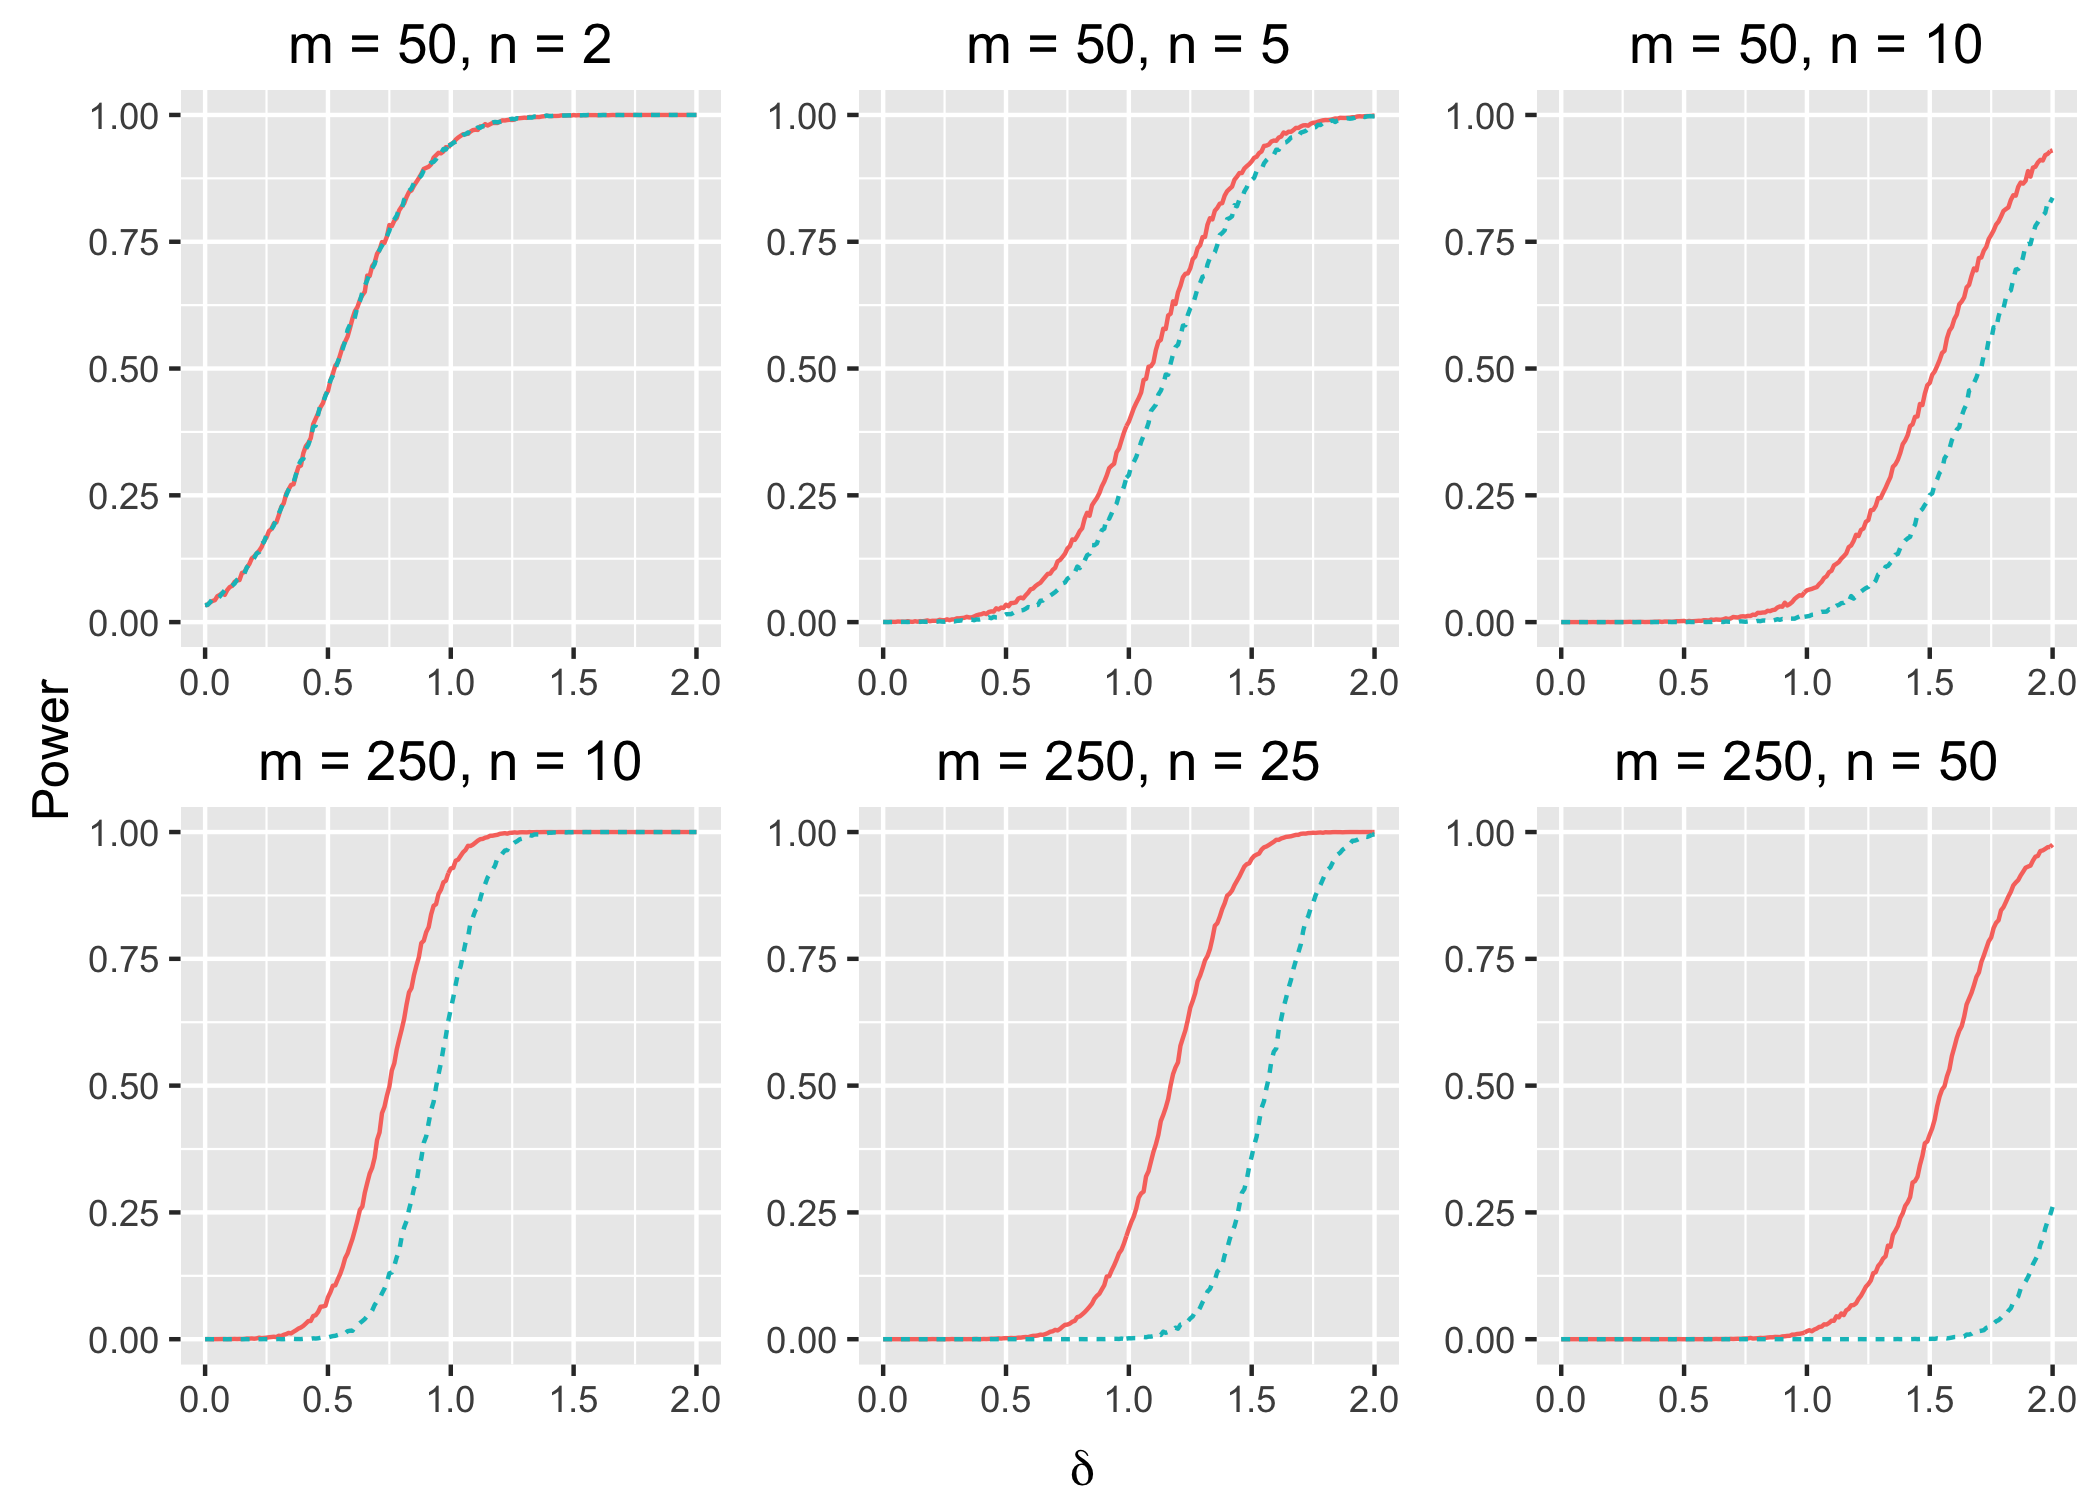
\includegraphics[width=\textwidth]{multinomial-power.pdf}

\begin{itemize}
	\item Our test performs better than \citet{Gupta:1967wg}
	\item Difference in performance increases with $m$ and $n$
	\item We attribute the improvement to our test adapting to the observations for winner and runner-up
\end{itemize}

\end{block}

\begin{block}{Selected References}

\small{
\bibliography{papers}
\bibliographystyle{abbrvnat}
\vspace{0.75in}
}

\end{block}

\end{column}

\end{columns}

\end{frame}

\end{document}
